\documentclass[letterpaper,12pt]{article}
\usepackage[utf8]{inputenc}

\usepackage{rotating}
\usepackage[top=1in, bottom=1in, left=1in, right=1in]{geometry}
\usepackage{graphicx}
\usepackage[numbers,square,sort&compress]{natbib}
\usepackage{setspace}
\usepackage[cdot,mediumqspace,]{SIunits}
\usepackage{hyperref}
\usepackage{mathtools}
\usepackage{url}
\usepackage{authblk}
\usepackage{placeins}
\usepackage{float}

\onehalfspacing
\title{Functional Analysis: Interpolation}
\author{Anita Bahmanyar}
\affil{\small {Student Number: 998909098}}
\affil{\small {anita.bahmanyar@mail.utoronto.ca}}
\date{December 19, 2014}

\usepackage{graphicx}

\renewcommand\thesubsection{\alph{subsection}}

\begin{document}

\maketitle

\section{Introduction}
Interpolation is generating a function based on a few points. This is similar to passing a curve from some points provided. Interpolation is useful in many cases. For instance, when we need the value of a function at many points but calculating those takes a long time, so we can use interpolation in that case. Also, sometimes  we do not need the function value at many points but instead we need to pass an array to the function but the function cannot get array as input due to Python built in functions such as quad function used to integrate. In that case, it is helpful to use interpolation.

\section{Interpolation Types}
\subsection{Linear Interpolation}
Linear interpolation is a method to fit a curve to the points using linear functions. if we know the coordinate of two points as $(x_0,y_0)$ and $(x_1,y_1)$, the linear interpolation between these two points would just be a straight line. The equation of a straight line is given by
\begin{equation}
y = y_0 +\frac{x-x_0}{x_1-x_0}
\end{equation}
This can be considered as the weighted average. The weights are inversely related to the distance from the end points to the unknown point; the closer point has more influence than the farther point. 



\subsection{Cubic Spline Interpolation}
Cubic spline interpolation is a more accurate and advanced way of fitting a curve to data points than the linear interpolation. We need to make sure the curves passing through the points have continuous second derivative at the knots. For this purpose, we need to use polynomials that are of order 3 or higher and that is where cubic spline name comes from.

\subsubsection{Mathematical Approach}
The aim is to fit a curve passing through points $(x_i,y_i)$ where $i=0,1,...,n$, so we interpolate between points $(x_{i-1},y_{i-1})$ and $(x_i,y_i)$ with polynomials $y_i = q_i(x)$.



In order to have continuous function at all the knots the following condition holds:
%equation
\begin{equation}
\frac{k_{i-1}}{x_i - x_{i-1}} +    \left (    \frac{1}{x_i - x_{i-1}} + \frac{1}{x_{i+1}-x_i} \right ) 2k_i + \frac{k_{i+1}}{x_{i+1}-x_i} = 3  \left(  \frac{y_i - y_{i-1}}{(x_i - x_{i-1})^2} + \frac{y_{i+1}-y_i}{( x_{i+1}-x_i )^2} \right)
\end{equation}
for $i=1,2,...,n-1$. This gives us $n-1$ equations including $k_0$, $k_1$, ..., $k_n$.

For the two knots at both ends, the condition is different and we have:
%equation
\begin{equation}
\frac{2}{x_1-x_0}k_0 + \frac{1}{x_1-x_0}k_1 = 3\frac{y_1-y_0}{(x_1-x_0)^2}
\end{equation}


%equation
\begin{equation}
\frac{1}{x_n-x_{n-1}}k_{n-1} + \frac{2}{x_n-x_{n-1}}k_n = 3\frac{y_n-y_{n-1}}{(x_n-x_{n-1})^2}
\end{equation}

These two equations give us 2 more equations and along with the previous $n-1$ equations we would have $n+1$ equations to solve for $k_0$,$k_1$,..,$k_n$ values. The cubic spline�s coefficients can be found by solving a tridiagonal linear system. 
%equation, matrix form
\begin{equation}
\begin{bmatrix}
a_{11} & a_{12} & &  &  & &\\ 
a_{21} & a_{22} & a_{23} & &  & &\\ 
 & a_{31} & a_{32} & a_{33} & & &\\
 &  & \ddots & \ddots & \ddots& &\\ 
 &  & & a_{n-1n-2}& a_{n-1n-1}&a_{n-1n}\\ 
 &  & & & a_{nn-1} & a_{nn}  
\end{bmatrix}
\begin{bmatrix}
k_0\\ 
k_1\\ 
k_2\\ 
\vdots\\ 
k_{n-1}\\
k_n\\
\end{bmatrix} = 
\begin{bmatrix}
b_0\\ 
b_1\\ 
b_2\\ 
\vdots\\ 
b_{n-1}\\
b_n \\
\end{bmatrix}
\end{equation}

Then having the values of $k_i$, we can calculate $a_i$ and $b_i$ values:
%equation
\begin{equation}
a_i = k_{i-1} (x_i-x_{i-1}) - (y_i - y_{i-1})
\end{equation}

%equation
\begin{equation}
b_i = -k_i (x_i - x_{i-1}) + (y_i - y_{i-1})
\end{equation}
and use these values to calculate $q_i$ values:

%equation
\begin{equation}
q_i = (1-t)y_{i_1} + ty_i + t(1-t) (a_i (1-t) +b_it)
\end{equation}
where t is:

%equation
\begin{equation}
t = \frac{x-x_{i-1}}{x_i - x_{i-1}}
\end{equation}

This will give us a function q for the points between each two knots, so we will have n different functions for the n+1 knots.


\subsubsection{Error Analysis}
The error in cubic spline interpolation is of order $O(h^4)$. The error would be the maximum difference between the value of the function we are approximating and our interpolated value. The error in cubic spline is given by:
\begin{equation}
\left | s-f \right | \sim \frac{5}{384}. \left | f^{(4)} \right |. h^4
\end{equation}
where $s-f$ is the difference between interpolated and the function value, $f^{(4)}$ is the value of fourth derivative of the function and h is the spacing between knots.
For example, if we do the interpolation on the function $y(x) = \sin(x)$ over the interval [0,3] with $h$= 0.1, what would the error be?
\\We know $f^{(4)}(x)$ = $\sin(x)$; therefore, $f^{(4)}(x) \leq$ 1. So the value of the error would be:
\\ $\frac{5}{384}.1.(0.1)^4$ $\approx$ $\frac{1}{768000} \approx 1.3 \times 10^{-6}$. This error is very small so the cubic spline interpolation is a good approximation of the function. 

Now to see how good it works, I have applied the code to do the interpolation for the function $\sin(x)$ in the interval [0,6.5] with 20 points, so $h$ = 0.325 here. So the error would be $\sim 1.46 \times 10^{-4}$. This is still quite a small error.

\section{Analysis}

\subsection{Code Analysis}
As you can see in figure 1, the Python built-in interpolation function does a better job in cubic spline interpolation than my code. The zoomed in figure shows that my interpolation is still very close to the actual function even though it differs a bit from the function and the python interpolated function.
%figure 1	
\FloatBarrier
\begin{figure}[H]
\centering
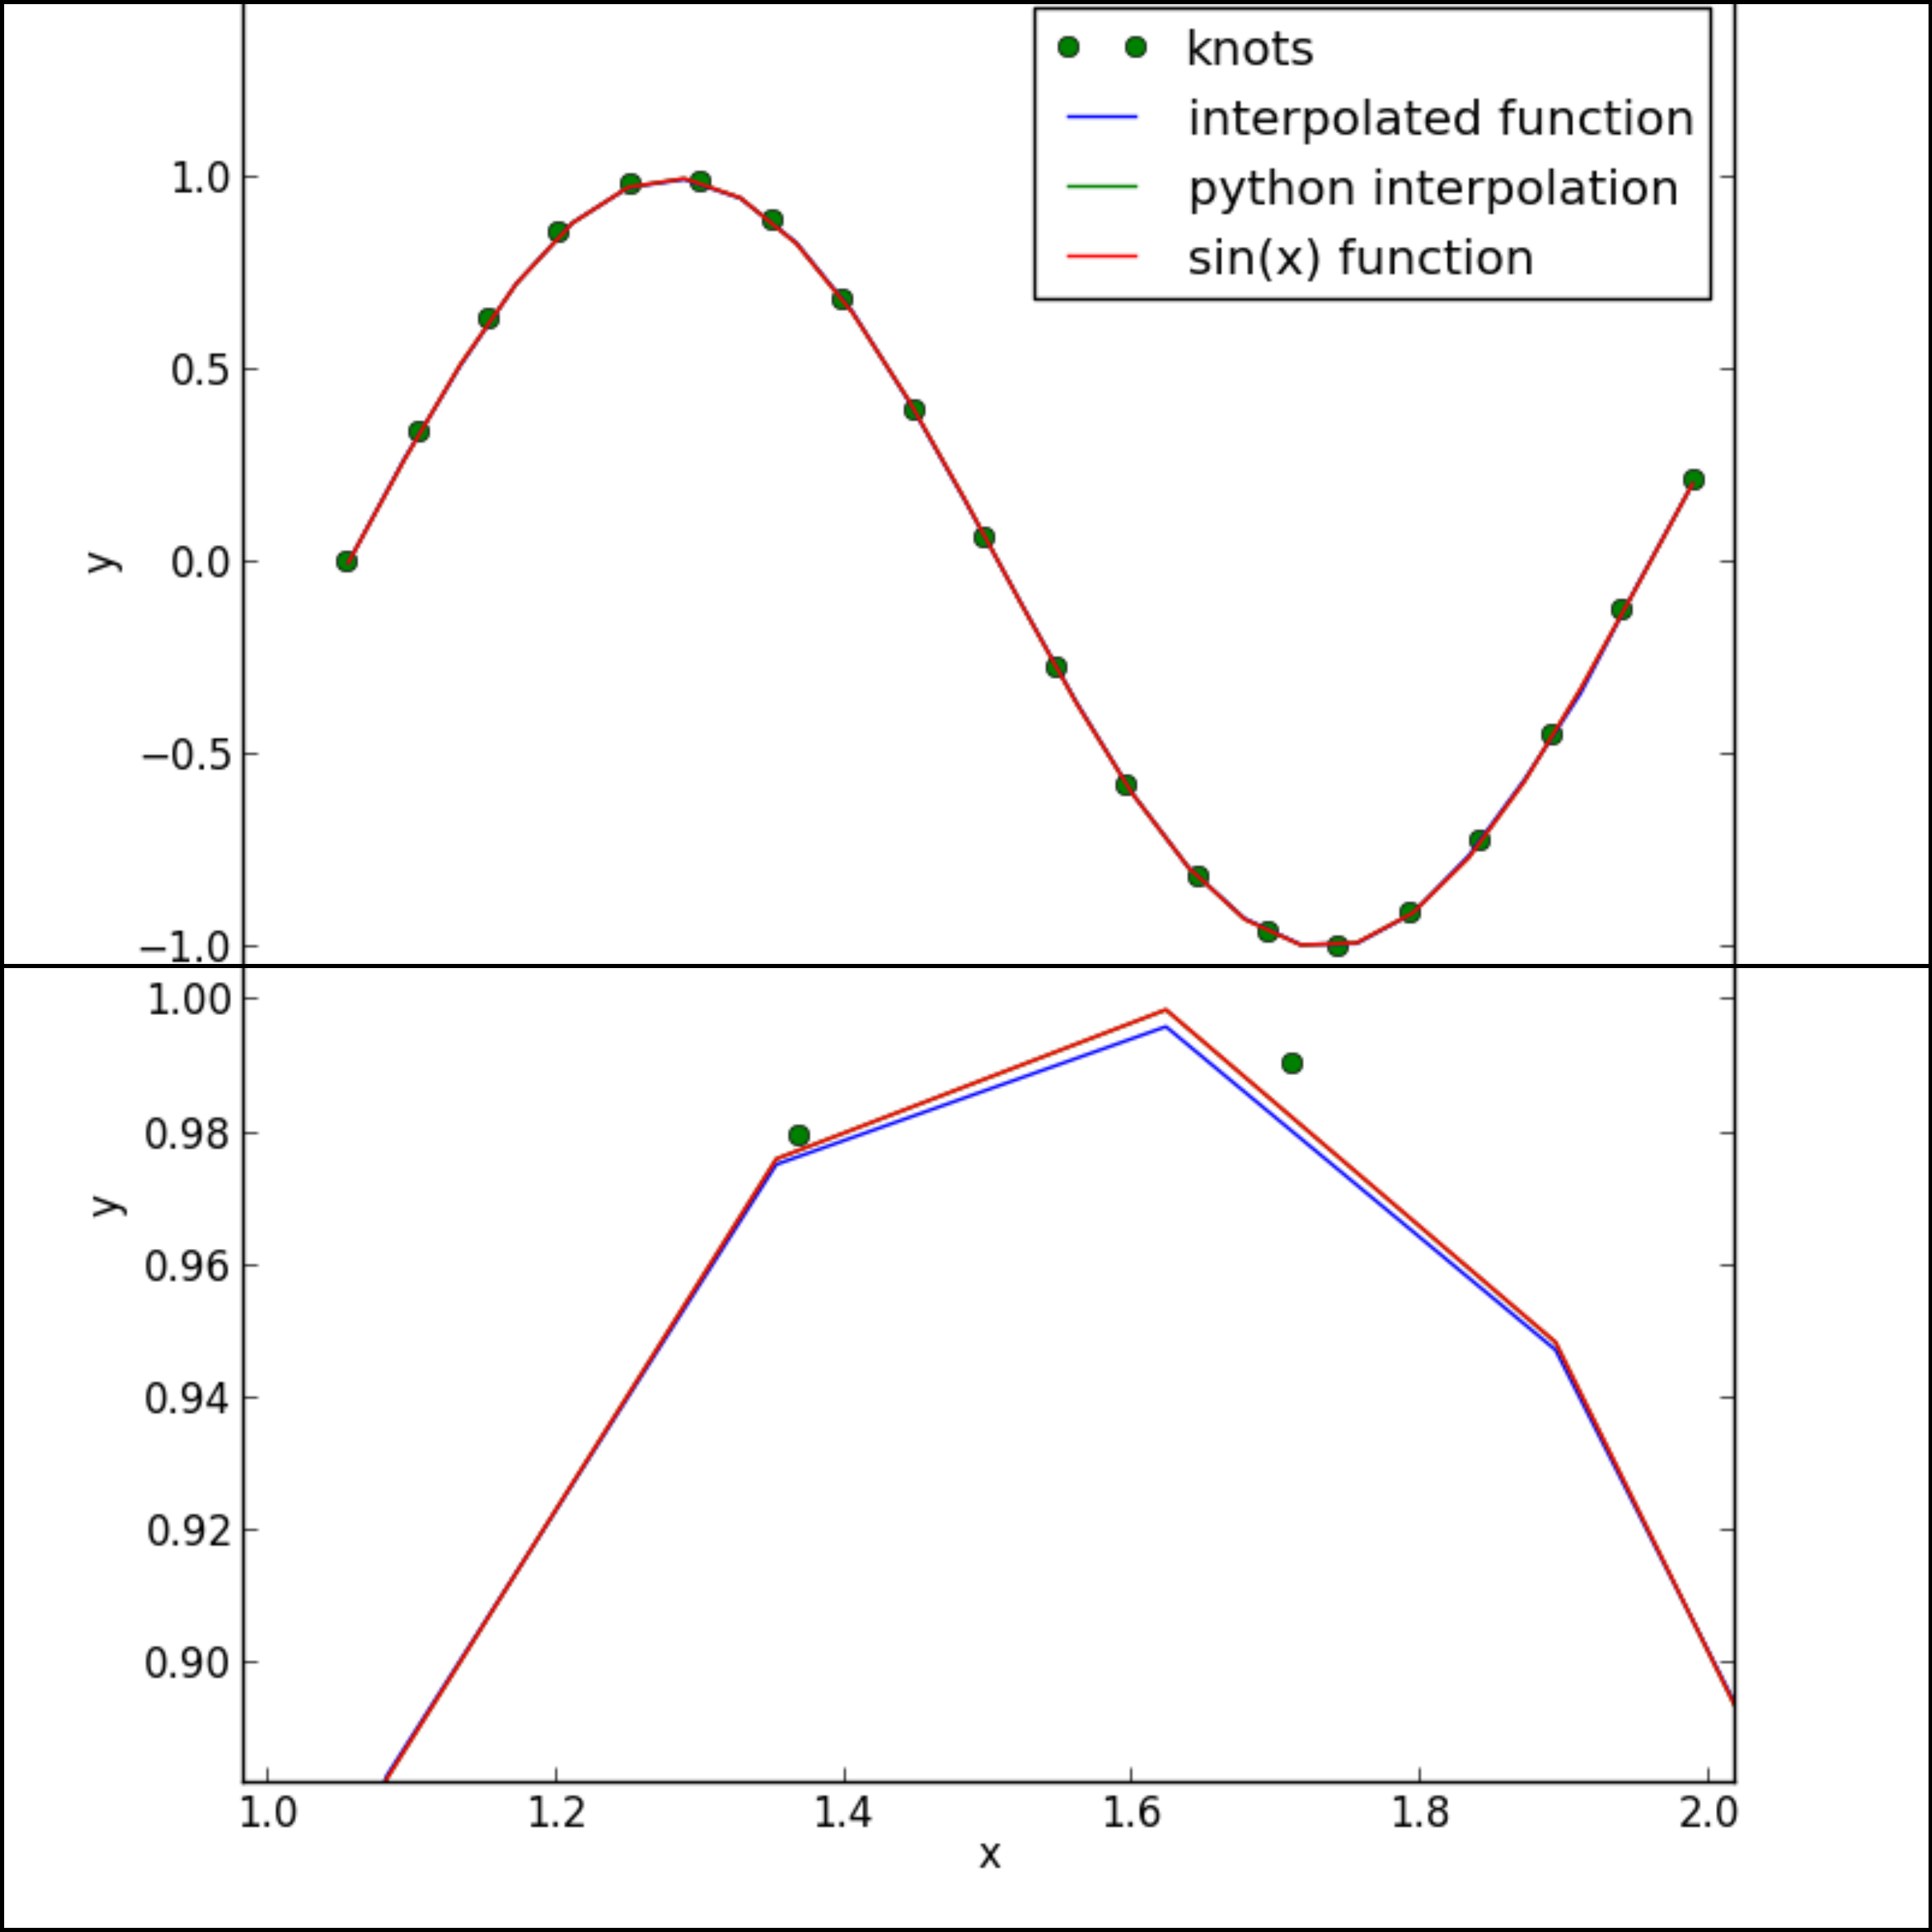
\includegraphics[scale=0.1]{cubic_compared_final.png}
\caption{Upper: Knots are shown in green dots, red is the actual sin(x) function and blue and green are my interpolated function and Python built-in interpolation function, respectively. Lower: Zoomed in version of the figure above. Python built-in function does a better job in cubic spline interpolation.}
\end{figure}
\FloatBarrier

\subsection{Bilinear Interpolation}

\end{document}


